% !TEX program = pdflatex
\documentclass[10pt,aspectratio=169]{beamer}

% ── Theme ──────────────────────────────────────────────────────────────
\usetheme{Madrid}
\usecolortheme{default}
\setbeamertemplate{navigation symbols}{}
\setbeamertemplate{footline}[frame number]

% Second-screen speaker notes (uncomment for presenting):
% \setbeameroption{show notes on second screen}

% ── Packages ───────────────────────────────────────────────────────────
\usepackage{graphicx}
\usepackage{booktabs}
\usepackage{tabularx}
\usepackage{listings}
\lstset{basicstyle=\footnotesize\ttfamily,breaklines=true}
\usepackage{tikz}
\usetikzlibrary{arrows.meta,positioning,shapes}
\usepackage{hyperref}
% ── Citation (reuse paper's bib) ──────────────────────────────────────
\usepackage[numbers]{natbib}
\bibliographystyle{IEEEtran}

% ── Convenience macros ─────────────────────────────────────────────────
\newcommand{\sectiondivider}[1]{%
  \begin{frame}[plain]
    \centering\vfill
    {\Huge\color{blue!60!black}#1}\par
    \vfill
  \end{frame}
}
\newcommand{\greencheck}{\textcolor{green!60!black}{\checkmark}}
\newcommand{\redcross}{\textcolor{red}{\ding{55}}}
\usepackage{pifont}

% Figure placeholder fallback: if file doesn't exist, draw a labelled box.
\newcommand{\incfig}[2][0.8\textwidth]{%
  \IfFileExists{#2}{%
    \includegraphics[width=#1]{#2}%
  }{%
    \fbox{\makebox[#1][c]{\shortstack{\small FIGURE TBD\\\tiny\detokenize{#2}}}}%
  }%
}
\newcommand{\incfigw}[2][\textwidth]{\incfig[#1]{#2}}

% ── Title ──────────────────────────────────────────────────────────────
\title{TrayGuard:\\What We Learned About Why Tray Errors Persist}
\subtitle{EC ENGR 180DW --- Final Design Review}
\author{Owen Fan, Matthew Li, Andy Ma, Jacob Moore, Qiyu Xin}
\date{\today}

\begin{document}

% ── Title slide ────────────────────────────────────────────────────────
\begin{frame}
  \titlepage
  \note{We're TrayGuard. We spent two quarters looking at why surgical trays
    arrive wrong or incomplete, and what a team like ours can actually do
    about it. The answer turned out to be more interesting --- and more
    frustrating --- than a camera-based fix.}
\end{frame}

% ── Outline ────────────────────────────────────────────────────────────
\begin{frame}{Roadmap}
  \tableofcontents
\end{frame}

% ======================================================================
%  SECTION 1: INTRODUCTION
% ======================================================================
\section{The Problem}
\sectiondivider{The Problem}

% ───────────────────────────────────────────────────────────────────────
% Slide 2: The problem by the numbers
% ───────────────────────────────────────────────────────────────────────
\begin{frame}{The Problem By The Numbers}
  \begin{columns}[T]
    \column{0.32\textwidth}
    \begin{block}{9 per 100 cases}
      \centering\small
      Alfred et al. (2021)\\
      3,900 defects in 41,799 cases\\
      \textbf{55\% at assembly}
    \end{block}
    \column{0.32\textwidth}
    \begin{block}{10 min avg delay}
      \centering\small
      Nichol et al. (2024)\\
      236 errors, 147 cases\\
      \textbf{\$6--9M/yr estimated cost}
    \end{block}
    \column{0.32\textwidth}
    \begin{block}{44\% wrong spec}
      \centering\small
      Zhu et al. (2019)\\
      398 errors in 33,839 packages\\
      \textbf{largest single category}
    \end{block}
  \end{columns}
  \vspace{0.5cm}
  \begin{alertblock}{}
    \centering
    These are recurring, measured operational failures --- not isolated accidents.
  \end{alertblock}
  \note{Three different methods --- tray defect analysis, direct OR observation,
    package inspection --- all find the same thing: instruments are missing,
    wrong, damaged, or swapped at rates that affect every shift, every hospital.
    When delays happen, they average 10 minutes per affected case. That doesn't
    sound huge until you multiply by thousands of cases a year.}
\end{frame}

% ======================================================================
%  SECTION 2: SYSTEMIC PROBLEM
% ======================================================================
\section{Why It Persists}
\sectiondivider{Why Tray Errors Persist}

% ───────────────────────────────────────────────────────────────────────
% Slide 3: What tray reconstruction requires
% ───────────────────────────────────────────────────────────────────────
\begin{frame}{What Tray Reconstruction Actually Requires}
  \begin{columns}[T]
    \column{0.48\textwidth}
    \centering
    \incfig[0.7\textheight]{figures/workstation_placeholder.pdf}
    \column{0.48\textwidth}
    \begin{itemize}
      \item Identify each instrument by sight (no labels)
      \item Match against a count sheet with \textbf{local names}
      \item Distinguish lookalikes (straight vs curved Mayo)
      \item Check for damage, wear, contamination
      \item Count correct quantities
      \item All under \textbf{production pressure}
    \end{itemize}
  \end{columns}
  \note{This is what tray reconstruction looks like. A technician gets a bin
    of returned instruments mixed together from the last surgery and has to
    identify each one, check for damage, match to a count sheet that may use
    local names, and place it correctly. No labels. Local names. Time pressure.}
\end{frame}

% ───────────────────────────────────────────────────────────────────────
% Slide 4: Fishbone RCA + structural drivers
% ───────────────────────────────────────────────────────────────────────
\begin{frame}{Six Root Causes}
  \centering
  \incfigw{figures/fishbone_placeholder.pdf}

  \vspace{0.3cm}
  \begin{columns}[T]
    \column{0.32\textwidth}
    \textbf{Three structural drivers:}
    \begin{enumerate}
      \item SPD evolved from materials management → \textbf{no licensure}
    \end{enumerate}
    \column{0.32\textwidth}
    \begin{enumerate}
      \setcounter{enumi}{1}
      \item Cost-center accounting → errors are \textbf{invisible}
    \end{enumerate}
    \column{0.32\textwidth}
    \begin{enumerate}
      \setcounter{enumi}{2}
      \item No information loop → errors \textbf{repeat}
    \end{enumerate}
  \end{columns}
  \note{We built a fishbone RCA across six categories: Product, Knowledge,
    Process, Information, Environment, Policy/Feedback. Underneath all six,
    three structural drivers explain why these problems persist. SPD evolved
    from materials management, not patient care, so there's no licensure.
    Hospital accounting treats SPD as a cost center -- error costs are
    invisible. And there's no information system to close the feedback loop.}
\end{frame}

% ───────────────────────────────────────────────────────────────────────
% Slide 5: Broken feedback loop
% ───────────────────────────────────────────────────────────────────────
\begin{frame}{The Broken Feedback Loop}
  \centering
  \incfigw{figures/feedback_loop_placeholder.pdf}

  \vspace{0.3cm}
  \begin{quote}
    \small
    ``Error reporting is cumbersome, human-dependent, delayed, and
    incomplete.'' --- Nichol et al.
  \end{quote}
  \note{This is the feedback loop that doesn't close. An instrument is missing
    during surgery. The scrub nurse fills an incident report on paper after the
    case. It reaches SPD management weeks later. By then nobody can connect it
    to the specific tray, shift, or training gap. So nothing changes. Even a
    perfect detector wouldn't fix this gap.}
\end{frame}

% ───────────────────────────────────────────────────────────────────────
% Slide 6: Seven solution categories
% ───────────────────────────────────────────────────────────────────────
\begin{frame}{We Evaluated Seven Solution Categories}
  \centering
  \small
  \begin{tabular}{lccc}
    \toprule
    Solution & Buildable? & Validatable? & Infra? \\
    \midrule
    CV tray checker       & No  & No  & Maybe \\
    Physical error-proofing & No  & No  & No \\
    Workflow redesign     & No  & No  & No \\
    Decision support      & Part & Part & Yes \\
    Task simplification   & No  & No  & No \\
    Accountability system & No  & No  & No \\
    \textbf{Training}     & \textbf{Yes} & \textbf{Yes} & \textbf{Yes} \\
    \bottomrule
  \end{tabular}
  \note{We mapped every intervention category in the literature and industry.
    Every one requires something we don't have: SPD deployment, policy
    authority, instrument inventory, or multi-stakeholder buy-in. Training is
    the only category buildable with printed cards and a laptop, validatable
    with a pre/post study, and creates durable infrastructure -- the local
    content module -- that future solutions need.}
\end{frame}

% ───────────────────────────────────────────────────────────────────────
% Slide 7: Training is not a cure
% ───────────────────────────────────────────────────────────────────────
\begin{frame}{Training is a Buildable Entry Point --- Not a Cure}
  \begin{columns}[T]
    \column{0.48\textwidth}
    \begin{exampleblock}{What training addresses}
      \begin{itemize}
        \item Measurable local tray knowledge
        \item Lookalike discrimination practice
        \item Pre/post learning evidence
      \end{itemize}
    \end{exampleblock}
    \column{0.48\textwidth}
    \begin{alertblock}{What training does NOT fix}
      \begin{itemize}
        \item Broken count sheets
        \item Staffing shortages
        \item Structural wage problems
        \item The broken feedback loop
      \end{itemize}
    \end{alertblock}
  \end{columns}
  \vspace{0.3cm}
  \begin{block}{}
    \centering
    Training is the one piece we can build and validate \textbf{now}.
  \end{block}
  \note{We need to be clear about what training does and doesn't do. It helps
    novices practice and produces measurable evidence. But it won't fix broken
    count sheets, solve staffing shortages, or close the feedback loop. Those
    are structural problems. Training is the one piece we can validate without
    a hospital partnership.}
\end{frame}

% ======================================================================
%  SECTION 3: CV EXPERIMENTS
% ======================================================================
\section{Why CV Alone Won't Work}
\sectiondivider{Why Computer Vision\\Alone Won't Work}

% ───────────────────────────────────────────────────────────────────────
% Slide 8: Experiment summary
% ───────────────────────────────────────────────────────────────────────
\begin{frame}{We Ran 7 Staged Detection Experiments}
  \centering
  \small
  \begin{tabular}{lrc}
    \toprule
    Experiment & Test & Key result \\
    \midrule
    Bright $\rightarrow$ dim   & Light tolerance & mAP50-95 = 0.781 \\
    Matte $\rightarrow$ reflective & Background & mAP50-95 = 0.759 \\
    Separated $\rightarrow$ overlay & Occlusion & \textbf{mAP50-95 = 0.389} \\
    Real instruments & Shape vs position & Per-class AP: 0.000--0.862 \\
    \bottomrule
  \end{tabular}
  \vspace{0.3cm}
  \begin{block}{}
    \centering
    Lavado baseline (clean data): \textbf{mAP50 = 0.990}\\
    Pipeline works --- the data doesn't generalize.
  \end{block}
  \note{We built a complete YOLO training pipeline. On a clean dataset we got
    mAP50 of 0.990. The pipeline works. The problem is what happens when you
    test on conditions SPD workstations actually present. Every variation cost
    accuracy. The biggest drop -- overlay layout -- produced mAP50-95 of 0.389.}
\end{frame}

% ───────────────────────────────────────────────────────────────────────
% Slide 9: Brightness
% ───────────────────────────────────────────────────────────────────────
\begin{frame}{Brightness Degradation}
  \centering
  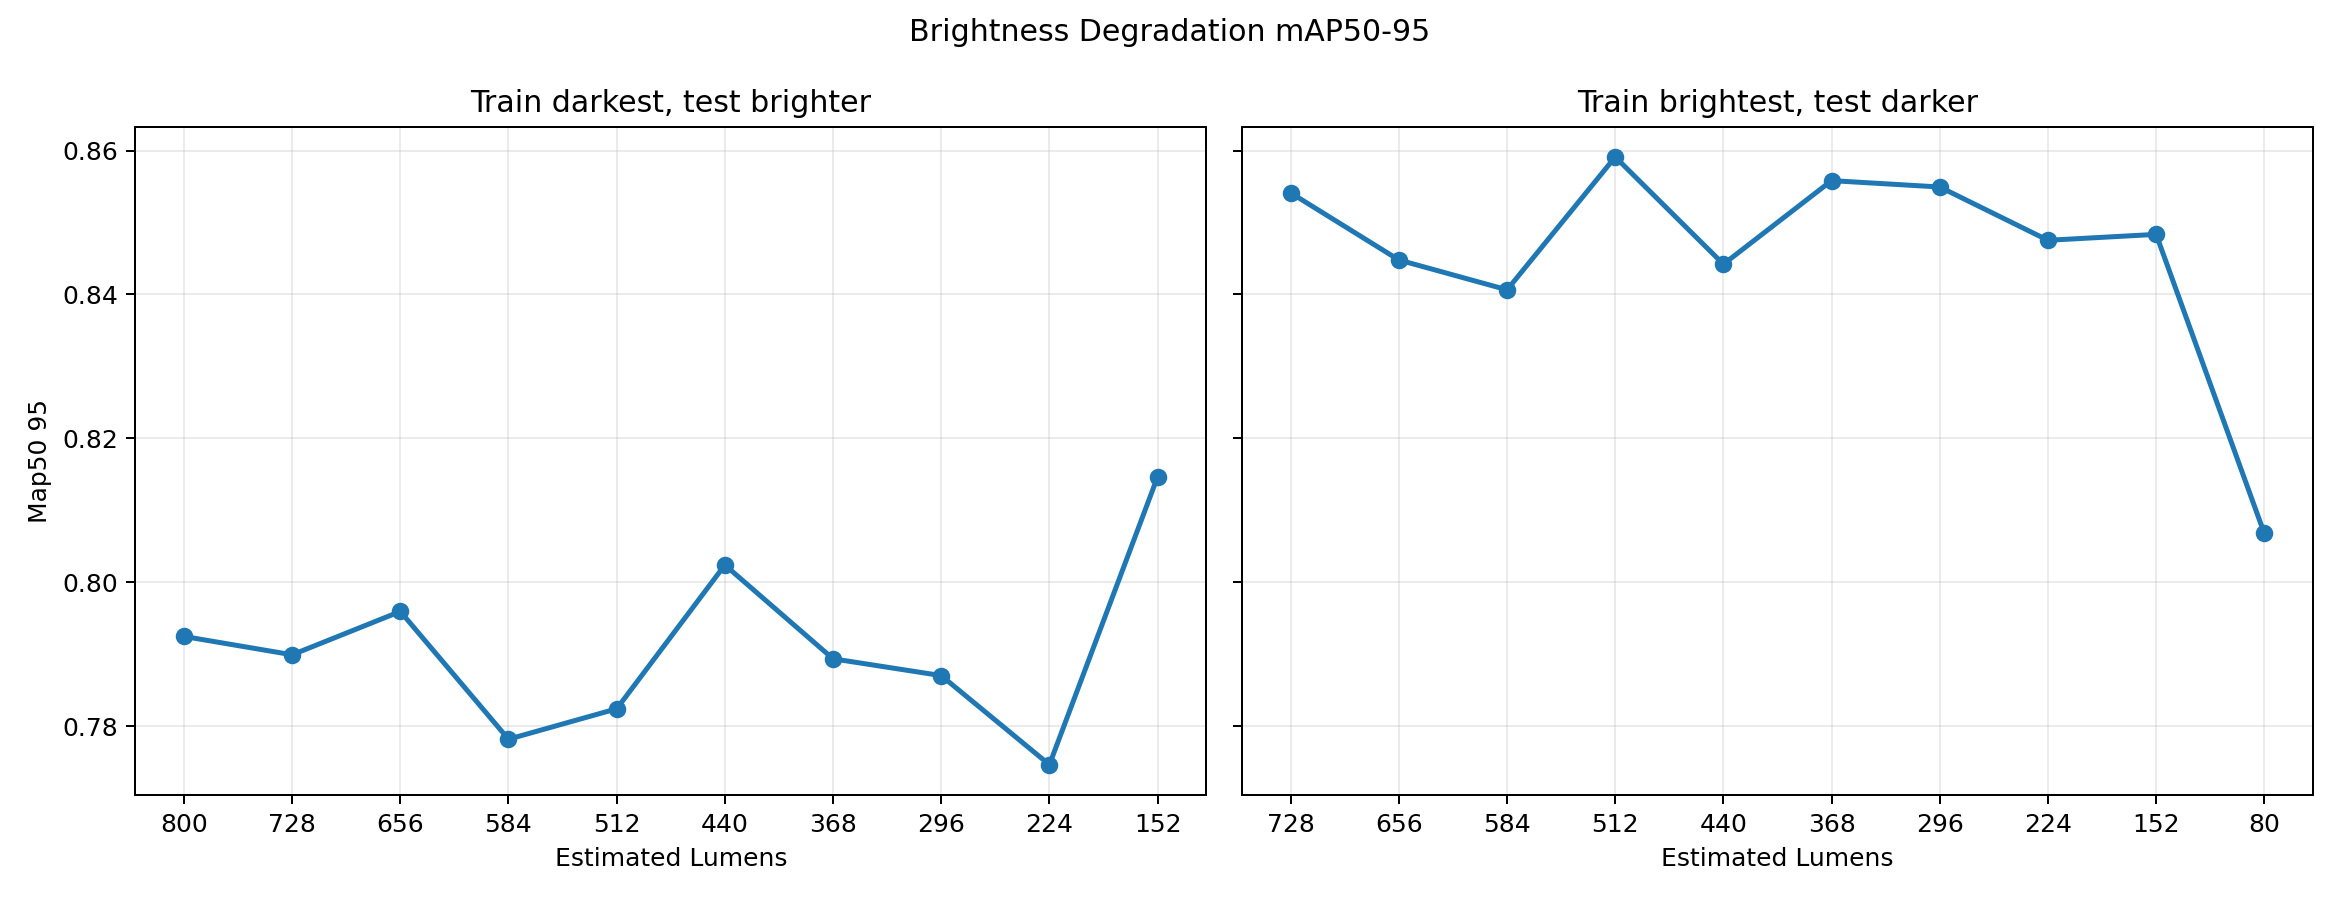
\includegraphics[width=0.8\textwidth]{figures/brightness_map50_95_panels.png}
  \note{This plot shows what happens as the light gap widens. Left: trained on
    darkest, tested on brighter. Right: trained on brightest, tested on dimmer.
    SPD lighting varies by workstation, time of day, fixture condition. Every
    variation costs detection reliability.}
\end{frame}

% ───────────────────────────────────────────────────────────────────────
% Slide 10: Occlusion
% ───────────────────────────────────────────────────────────────────────
\begin{frame}{Occlusion Is the Dealbreaker}
  \begin{columns}[T]
    \column{0.48\textwidth}
    \centering
    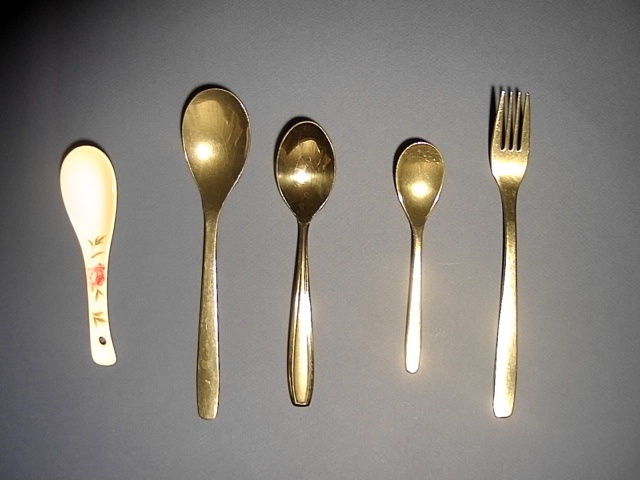
\includegraphics[width=\textwidth]{figures/separated_layout_example.jpg}\\
    \tiny Separated layout (training)
    \column{0.48\textwidth}
    \centering
    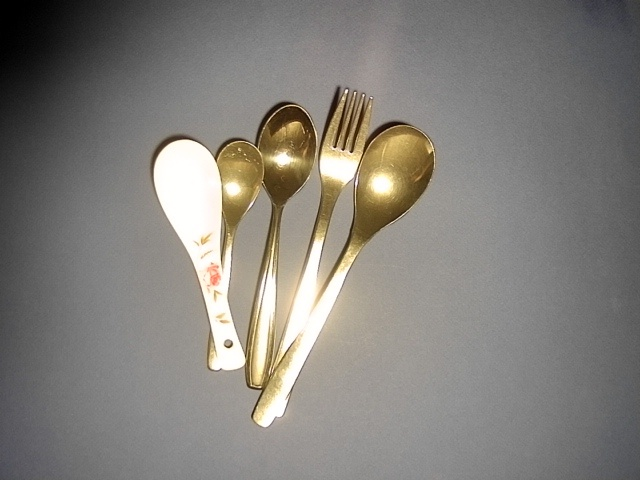
\includegraphics[width=\textwidth]{figures/overlay_layout_example.jpg}\\
    \tiny Overlay layout (test)
  \end{columns}
  \vspace{0.2cm}
  \centering
  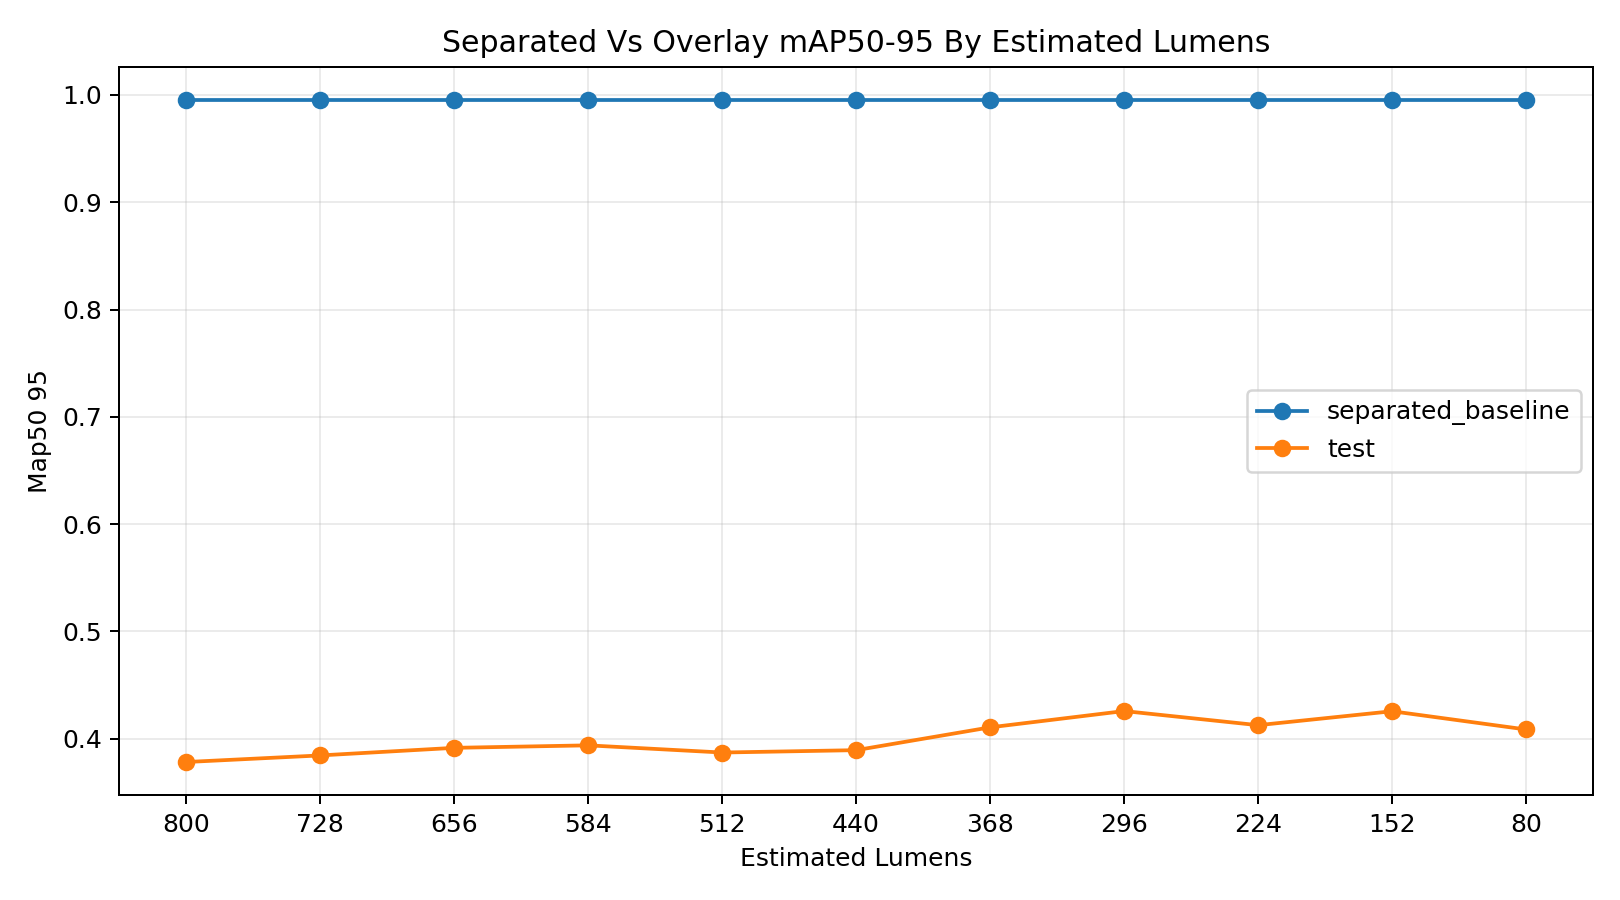
\includegraphics[width=0.6\textwidth]{figures/overlay_map50_95.png}
  \note{Left: separated layout -- what you'd train on. Right: overlay -- what
    a real tray looks like. When we trained separated and tested on overlay,
    mAP50-95 dropped from 0.995 to 0.389. You'd need to ask the technician to
    rearrange before scanning, which defeats the purpose.}
\end{frame}

% ───────────────────────────────────────────────────────────────────────
% Slide 11: Position-cue confounding
% ───────────────────────────────────────────────────────────────────────
\begin{frame}{Real Instruments: The Model Learned Position, Not Shape}
  \begin{columns}[T]
    \column{0.45\textwidth}
    \centering
    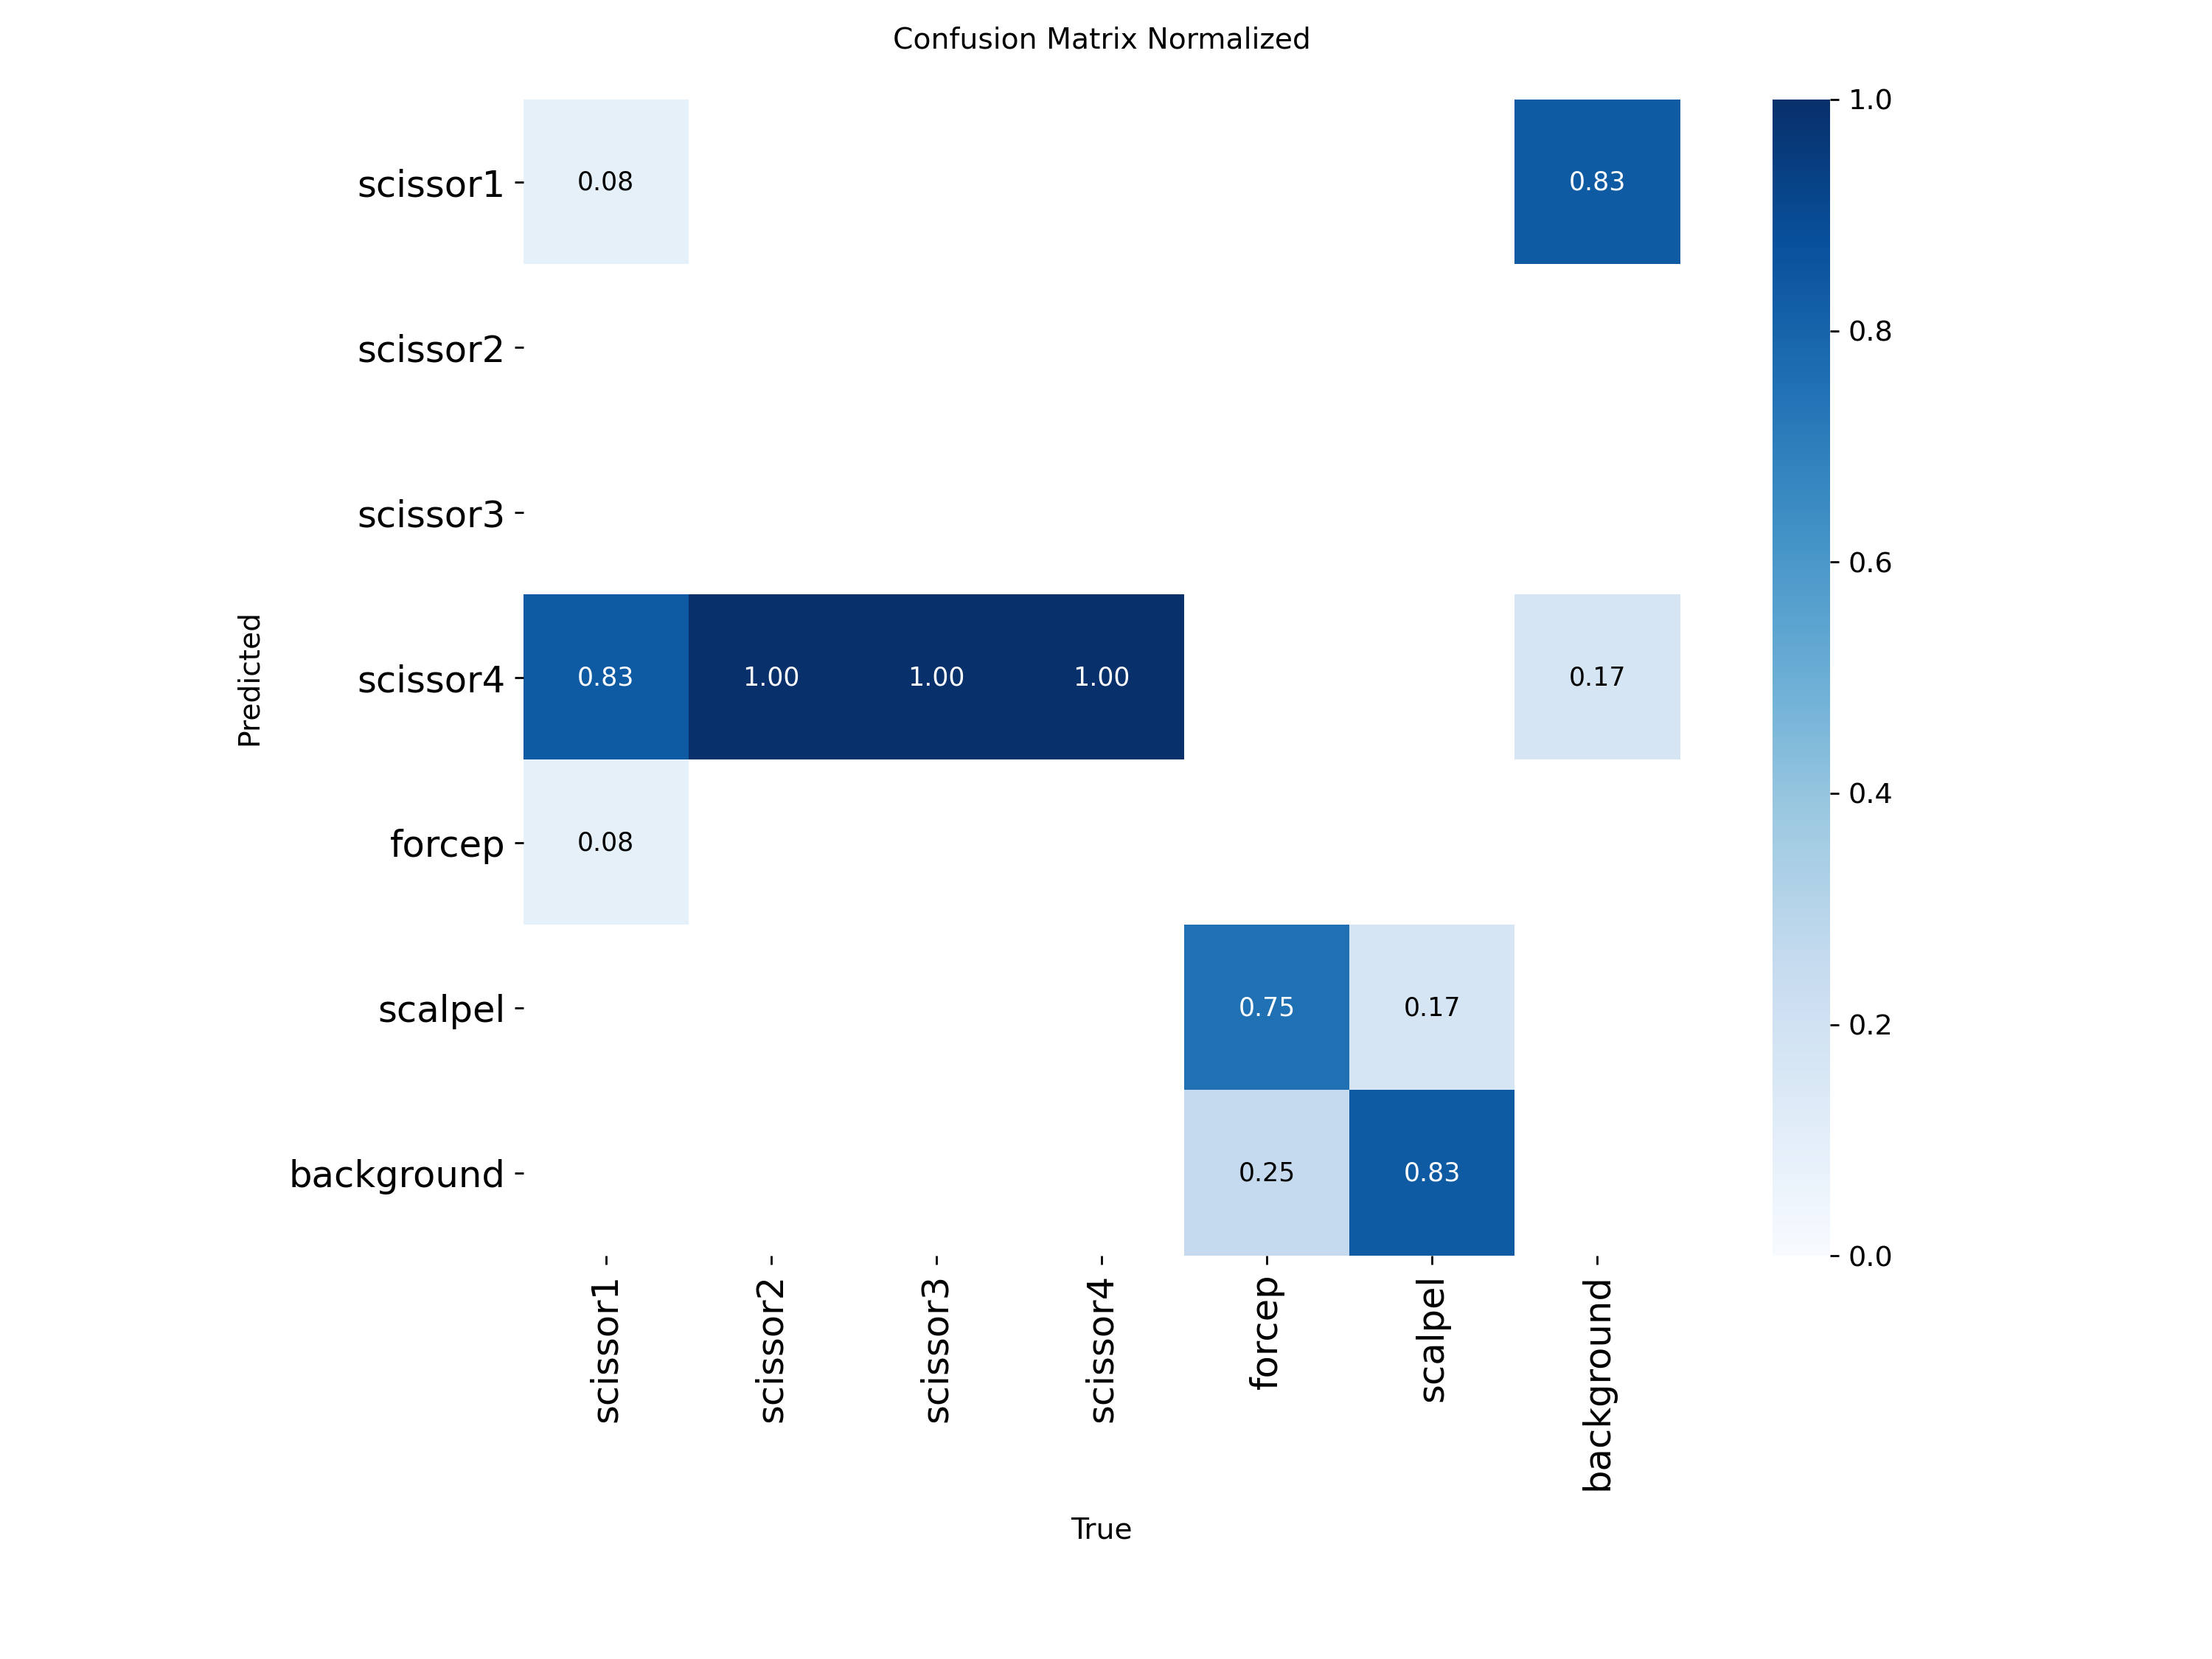
\includegraphics[width=\textwidth]{figures/confusion_matrix_normalized.png}
    \column{0.45\textwidth}
    \centering
    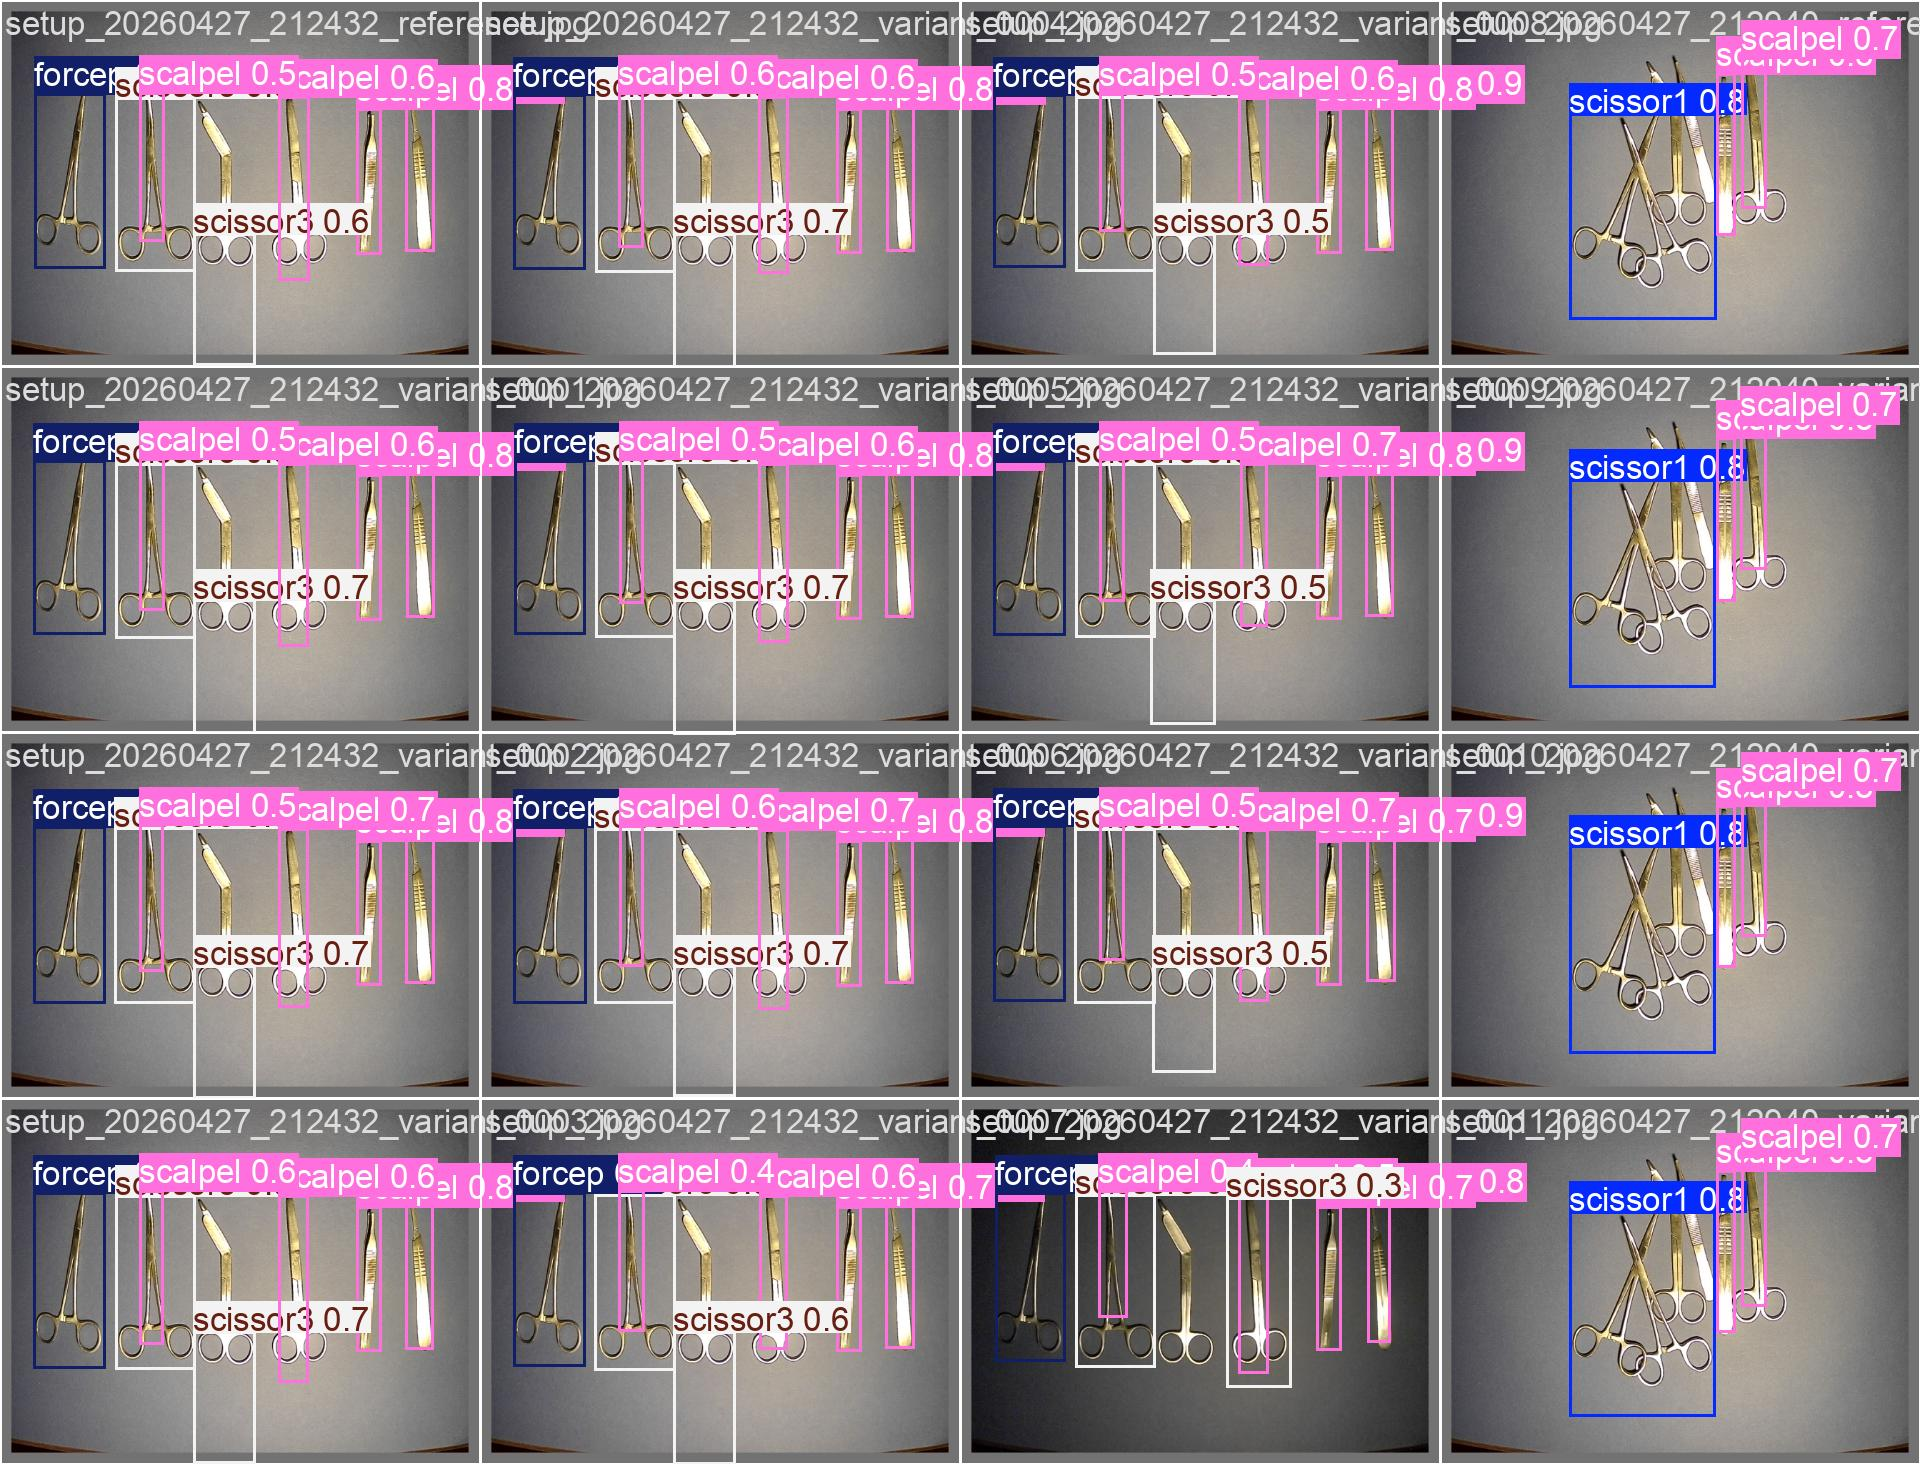
\includegraphics[width=\textwidth]{figures/val_batch0_pred.jpg}
  \end{columns}
  \vspace{0.2cm}
  \centering
  \small
  \begin{tabular}{lcc}
    \toprule
    Split & Surviving classes & Zero AP \\
    \midrule
    Matte $\rightarrow$ reflective & scissor2, forcep, scalpel & scissor1/3/4 \\
    Reflective $\rightarrow$ matte & \textbf{scalpel only} & all others \\
    Shape similarity & scissor1, scissor4 & scissor2/3, forcep \\
    \bottomrule
  \end{tabular}
  \note{This is diagnostic. Per-class AP ranges from 0.000 to 0.862 depending
    on the split. Different classes survive in different splits because the
    model memorizes positions, not shapes. The only class that transfers is
    scalpel -- the most visually distinct. This isn't fixable with more data
    alone; you'd need randomized positions.}
\end{frame}

% ───────────────────────────────────────────────────────────────────────
% Slide 12: CV validation burden
% ───────────────────────────────────────────────────────────────────────
\begin{frame}{The Cumulative Lesson}
  \begin{block}{What a deployment-grade CV system still needs}
    \begin{itemize}
      \item[$\times$] Site-specific training data (instruments, lighting, layouts)
      \item[$\times$] Cross-manufacturer validation \cite{kienle-et-al-2025}
      \item[$\times$] Open-set rejection (unknown objects = false positives)
      \item[$\times$] Human-in-the-loop for every uncertain case
      \item[$\times$] Workflow integration in live SPD
      \item[$\times$] Regulatory / device policy / privacy review
    \end{itemize}
  \end{block}
  \vspace{0.3cm}
  \begin{exampleblock}{}
    \centering
    The training path doesn't need any of this for a first study.
  \end{exampleblock}
  \note{CV works in matched controlled conditions and degrades under every SPD
    variation. A deployment-grade system needs site-specific data for every
    hospital, cross-manufacturer validation, open-set rejection, human review,
    and regulatory clearance. We cannot responsibly build that in a quarter.
    The pivot was driven by this evidence.}
\end{frame}

% ======================================================================
%  SECTION 4: TRAINING DESIGN
% ======================================================================
\section{The Training Path}
\sectiondivider{Why Training Is the\\Best Entry Point}

% ───────────────────────────────────────────────────────────────────────
% Slide 13: CV and training are complementary
% ───────────────────────────────────────────────────────────────────────
\begin{frame}{CV and Training Are Complementary, Not Competing}
  \centering
  \incfigw{figures/complementary_placeholder.pdf}

  \vspace{0.3cm}
  \begin{block}{}
    \centering
    The module is the durable artifact. The training loop proves the module
    works. The module then enables CV.
  \end{block}
  \note{Building a CV tray checker without a training layer means no ground
    truth. You don't know the correct names, aliases, or lookalike pairs.
    The training loop builds and validates all of that at low cost. Once you
    have a validated module, that same data feeds any future CV system.}
\end{frame}

% ───────────────────────────────────────────────────────────────────────
% Slide 14: Tray module schema
% ───────────────────────────────────────────────────────────────────────
\begin{frame}[fragile]{The Durable Artifact: Tray Module Schema}
  \begin{columns}[T]
    \column{0.55\textwidth}
    \begin{lstlisting}
{
  "id": "mayo_scissors_straight_55",
  "display_name": "Straight Mayo, 5.5 in",
  "aliases": ["straight Mayo",
              "suture scissors"],
  "distinguishing_features": [
    "Heavy straight blades"
  ],
  "common_confusions": [
    "mayo_scissors_curved_55"
  ],
  "apriltag_id": 12,
  "study_prompts": [ ... ]
}
    \end{lstlisting}
    \column{0.42\textwidth}
    \begin{itemize}
      \item Mirrors real count-sheet fields
      \item Adds aliases, lookalikes, prompts
      \item File-backed, versioned
      \item \textbf{Software is throwaway.}
      \item \textbf{Schema survives.}
    \end{itemize}
  \end{columns}
  \note{This is the durable output. The fields mirror real count-sheet
    structure from Stryker's published sheets. The software prototype is
    throwaway -- future teams will choose their own stack -- but this schema
    captures the local tray knowledge that any solution needs.}
\end{frame}

% ───────────────────────────────────────────────────────────────────────
% Slide 15: Printed cards
% ───────────────────────────────────────────────────────────────────────
\begin{frame}{Printed Cards: How It Works Physically}
  \begin{columns}[T]
    \column{0.48\textwidth}
    \centering
    \textbf{Front (assessment)}\\
    \incfig[0.5\textheight]{figures/card_front_placeholder.pdf}
    \column{0.48\textwidth}
    \centering
    \textbf{Back (study)}\\
    \incfig[0.5\textheight]{figures/card_back_placeholder.pdf}
  \end{columns}
  \vspace{0.2cm}
  \begin{block}{}
    \centering
    Neutral front prevents answer leakage. Tag ID maps to instrument ID.
  \end{block}
  \note{Each instrument gets a printed card. The front has an AprilTag with no
    text, so during a test the learner can't read the answer off the card. The
    back has name, aliases, and features for study mode. The learner places
    cards on a table, the camera detects them, and the scoring engine compares
    against the tray template.}
\end{frame}

% ───────────────────────────────────────────────────────────────────────
% Slide 16: Scoring categories
% ───────────────────────────────────────────────────────────────────────
\begin{frame}{The Scoring Architecture: 5 Error Categories}
  \centering
  \small
  \begin{tabular}{lll}
    \toprule
    Category & Definition & Example \\
    \midrule
    Correct & Right item, right count & 1 scalpel handle \\
    Missing & Required item not selected & No Kelly clamp \\
    Wrong & Item not on tray list & Retractor not in this tray \\
    Extra & Distractor selected & Item from different tray \\
    Misidentified & Right class, wrong variant & Curved instead of straight \\
    Wrong count & Right item, wrong quantity & 2 Kellys, need 4 \\
    \bottomrule
  \end{tabular}
  \vspace{0.3cm}
  \begin{itemize}
    \item Maps to literature error categories \cite{alfred-et-al-2021, zhu-et-al-2019, nichol-et-al-2024}
    \item Can separate \textit{what} improved (fewer misses? fewer lookalikes?)
  \end{itemize}
  \note{These six categories map directly to the literature. Zhu's 44\% wrong
    specification -- that's misidentified. Alfred's missing, wrong, extra,
    damaged -- we capture all of them. When a learner improves, we can say
    which type of error they reduced.}
\end{frame}

% ───────────────────────────────────────────────────────────────────────
% Slide 17: Confidence capture
% ───────────────────────────────────────────────────────────────────────
\begin{frame}{Confidence Capture}
  \centering
  \incfigw{figures/confidence_mockup_placeholder.pdf}

  \vspace{0.3cm}
  \begin{columns}[T]
    \column{0.48\textwidth}
    \begin{alertblock}{High-confidence error}
      Learner was sure but wrong\\
      Targeted feedback needed
    \end{alertblock}
    \column{0.48\textwidth}
    \begin{exampleblock}{Low-confidence correct}
      Learner was unsure but right\\
      Fragile knowledge, needs reinforcement
    \end{exampleblock}
  \end{columns}
  \note{After each tray sort, the learner rates confidence. This separates
    two failure modes: high-confidence errors (overconfidence, hardest to
    correct) and low-confidence correct answers (fragile knowledge). Both
    are visible in the export.}
\end{frame}

% ───────────────────────────────────────────────────────────────────────
% Slide 18: Learning loop
% ───────────────────────────────────────────────────────────────────────
\begin{frame}{The 7-Step Learning Loop}
  \centering
  \incfigw{figures/learning_loop_placeholder.pdf}

  \vspace{0.2cm}
  \begin{block}{}
    Pre-test (baseline) $\rightarrow$ Study cards $\rightarrow$ Quiz
    $\rightarrow$ Practice sort $\rightarrow$ Post-test $\rightarrow$ Export
  \end{block}
  \note{Each step has an evidence-based role. Pre/post use parallel variants
    so learners can't memorize exact layouts. Study cards are prompt-before-
    reveal -- retrieval practice, not passive review. Practice sort gives
    immediate error feedback. The full loop takes 45-60 minutes.}
\end{frame}

% ───────────────────────────────────────────────────────────────────────
% Slide 19: Research question
% ───────────────────────────────────────────────────────────────────────
\begin{frame}{The Research Question}
  \begin{center}
    \vfill
    \Large
    How can a local tray training and assessment system help novice users
    improve their ability to detect missing, wrong, extra, misidentified,
    or miscounted instruments before supervised SPD work?
    \vfill
  \end{center}
  \begin{exampleblock}{}
    \centering
    That question is narrow, testable, and honest about what we can claim.
  \end{exampleblock}
  \note{That's the research question this design answers. Not "does TrayGuard
    reduce OR delays." Not "does it certify competence." It's: can a novice
    improve on a simulated tray task after retrieval-centered practice? That's
    a question we can answer.}
\end{frame}

% ======================================================================
%  SECTION 5: FUTURE WORK
% ======================================================================
\section{Future Validation}
\sectiondivider{What a Future Team Should Do}

% ───────────────────────────────────────────────────────────────────────
% Slide 20: Study ladder
% ───────────────────────────────────────────────────────────────────────
\begin{frame}{The Study Ladder}
  \centering
  \incfigw{figures/study_ladder_placeholder.pdf}

  \vspace{0.3cm}
  \begin{alertblock}{}
    Kirkpatrick Level 2 target. Level 3--4 require future validation.
  \end{alertblock}
  \note{Each step validates a different piece of the evidence chain. Step 1
    ensures the measurement tool works. Step 2 tests learning mechanism. Step 3
    checks retention at 7 days. Step 4 brings in an expert. Only after all four
    should someone invest in an SPD pilot.}
\end{frame}

% ───────────────────────────────────────────────────────────────────────
% Slide 21: Study 1 novice
% ───────────────────────────────────────────────────────────────────────
\begin{frame}{Study 1: Novice Pre/Post Design}
  \centering
  \small
  \begin{tabular}{lrl}
    \toprule
    Segment & Time & Activity \\
    \midrule
    Consent + intake & 3--5 min & Background \\
    Pre-test tray sort & 5--8 min & No hints, no feedback \\
    Retrieval cards & 10--12 min & Prompt-before-reveal \\
    Quiz & 5--8 min & With confidence \\
    Practice sort & 8--10 min & Error feedback \\
    Post-test & 5--8 min & Parallel variant, no hints \\
    Photo-ID test & 5--7 min & Convergent validity \\
    \bottomrule
  \end{tabular}
  \vspace{0.3cm}
  \begin{block}{}
    $\mathbf{n = 8\text{--}12}$ novices, one 60-min session, within-subject
  \end{block}
  \note{The novice study uses a within-subject pre/post design. 8-12
    participants with no SPD experience. Primary measures: pre/post accuracy,
    error categories, duration, confidence. Convergent photo-ID test
    correlates tray accuracy with photo identification (target r $\ge$ 0.50).}
\end{frame}

% ───────────────────────────────────────────────────────────────────────
% Slide 22: Delayed retention
% ───────────────────────────────────────────────────────────────────────
\begin{frame}{Study 2: Delayed Retention}
  \centering
  \incfigw{figures/retention_placeholder.pdf}

  \vspace{0.3cm}
  \begin{columns}[T]
    \column{0.32\textwidth}
    \textbf{Criterion 1}\\
    $\ge$ 50\% of gain retained
    \column{0.32\textwidth}
    \textbf{Criterion 2}\\
    Accuracy $>$ 5pp above baseline
    \column{0.32\textwidth}
    \textbf{Criterion 3}\\
    $\ge$ 70\% return rate
  \end{columns}
  \vspace{0.2cm}
  \begin{alertblock}{}
    If these fail, the claim reverts to ``immediate learning only.''
  \end{alertblock}
  \note{Same-day post-test can't be called retention. Bell et al. showed
    medical gains decay measurably within 7 days. We require three
    falsification criteria: retain half the gain, stay above baseline, and
    70\% return rate. If these fail, we report immediate learning only.}
\end{frame}

% ───────────────────────────────────────────────────────────────────────
% Slide 23: Expert review
% ───────────────────────────────────────────────────────────────────────
\begin{frame}{Study 3: Expert Review}
  \begin{itemize}
    \item[\textbf{Q}] Are instrument names and aliases correct for local practice?
    \item[\textbf{Q}] Are counts and distractors plausible for training?
    \item[\textbf{Q}] Are lookalike pairs educationally meaningful?
    \item[\textbf{Q}] Are feedback messages misleading or safe?
    \item[\textbf{Q}] Would the weak-item report help target coaching?
  \end{itemize}
  \vspace{0.3cm}
  \begin{block}{}
    \centering
    The main weakness of a student-built module is \textbf{content validity}.
    Expert review closes that gap.
  \end{block}
  \note{We don't work in an SPD. An instructor or SPD educator needs to
    review names, counts, distractors, and feedback. If they say the module
    is plausible, we proceed to an SPD pilot. If they find problems, we fix
    them first.}
\end{frame}

% ───────────────────────────────────────────────────────────────────────
% Slide 24: Go/no-go
% ───────────────────────────────────────────────────────────────────────
\begin{frame}{Go/No-Go Decision}
  \centering
  \incfigw{figures/gonogo_placeholder.pdf}

  \vspace{0.3cm}
  \begin{block}{}
    \centering
    Study passes $\rightarrow$ SPD pilot is justified.\\
    Study fails $\rightarrow$ problem may be harder than training alone.
  \end{block}
  \note{If the novice study shows learning, retention persists, and content
    is plausible, then investing in an SPD pilot is justified. If it fails,
    the problem may be harder than training alone can solve -- and that's
    useful evidence too.}
\end{frame}

% ======================================================================
%  SECTION 6: CONCLUSION
% ======================================================================
\section{Conclusion}
\sectiondivider{Conclusion}

% ───────────────────────────────────────────────────────────────────────
% Slide 25: Know / don't know
% ───────────────────────────────────────────────────────────────────────
\begin{frame}{What We Know and What We Don't}
  \begin{columns}[T]
    \column{0.48\textwidth}
    \begin{exampleblock}{What we know}
      \begin{itemize}
        \item Tray errors are systemic and well-documented
        \item CV alone has too high a validation burden
        \item Training is the buildable entry point
        \item The module schema is durable infrastructure
        \item The study ladder has falsification criteria
      \end{itemize}
    \end{exampleblock}
    \column{0.48\textwidth}
    \begin{alertblock}{What we can't claim (yet)}
      \begin{itemize}
        \item Training transfers to real SPD work
        \item System works for experienced techs
        \item It reduces OR delays
        \item CV is deployment-ready
        \item Same-day gains persist (Study 2)
      \end{itemize}
    \end{alertblock}
  \end{columns}
  \note{This sums up what we accomplished. We didn't build a deployable
    product. We built an evidence-backed argument for the right starting
    point, designed the measurement infrastructure, and left a testable
    protocol.}
\end{frame}

% ───────────────────────────────────────────────────────────────────────
% Slide 26: Honest handoff
% ───────────────────────────────────────────────────────────────────────
\begin{frame}{The Honest Handoff}
  \begin{center}
    \vfill
    \Large
    Our project found that this problem is harder and more systemic than\\
    any single technical fix can address.\\
    \vspace{0.5cm}
    Our contribution is documenting \textit{why}, and giving the next team\\
    a validated starting point --- not a finished product.
    \vfill
  \end{center}
  \vspace{0.3cm}
  \begin{block}{}
    \centering\large
    The study is designed. The schema is defined. The scoring is tested.\\
    \textbf{Run the study.}
  \end{block}
  \note{We started thinking we'd build a camera that catches tray errors. We
    ended up understanding that tray errors are a system problem rooted in how
    the SPD workforce is structured, funded, and connected to the OR. A camera
    can't fix that. Training alone can't fix wage stagnation or staffing gaps.
    But a training loop can create the infrastructure every future solution
    needs. Our honest recommendation: take the schema, protocol, and criteria.
    Run the study.}
\end{frame}

% ── References ─────────────────────────────────────────────────────────
\begin{frame}[allowframebreaks]{References}
  \bibliography{trayguard_refs}
\end{frame}

\end{document}
